\section{Entwurf eines Fuzzy-Reglers}

\subsection{Grundlegende Idee und Begründung}

Im Verlauf des Projekts entstand die Idee, zusätzlich einen Fuzzy-Regler zu entwerfen und die Fahrten alternativ über diesen zu realisieren. Da Fuzzy-Regler nicht auf einem exakten linearen Modell des Roboters basieren, sondern mit linguistischen Regeln arbeiten, wurde dieser Regleransatz als sinnvoll erachtet. Anstatt den analytischen Zusammenhang zwischen Regelabweichung und Stellgröße vollständig herzuleiten, wird das Reglerverhalten durch Zugehörigkeitsfunktionen und eine Regelbasis beschrieben. 

Ein wesentlicher Vorteil des Fuzzy-Reglers besteht darin, dass sich sein Verhalten durch die gezielte Anpassung weniger, physikalisch nachvollziehbarer Parameter einstellen lässt. Bereits kleine Änderungen der Parameter der Zugehörigkeitsfunktionen ermöglichen eine systematische Anpassung des Fahrverhaltens an unterschiedliche Anforderungen, ohne die grundlegende Reglerstruktur verändern zu müssen. Ziel war es daher, den Regler möglichst allgemein auszulegen, sodass er als Baustein mit geringem Parametrieraufwand an neue Randbedingungen oder geänderte Anforderungen angepasst werden kann


Darüber hinaus wollte unsere Gruppe praktische Erfahrungen mit Fuzzy-Reglern sammeln. Zwar war bereits theoretisches Wissen zu dieser Reglerstruktur vorhanden, praktische Erfahrungen lagen jedoch noch nicht vor. Das Projekt bot daher die Möglichkeit, diese Wissenslücke in einem kontrollierten Umfeld zu schließen und Erfahrungen im Entwurf sowie in der Implementierung eines Fuzzy-Reglers zu sammeln. Ziel war es daher, einen Fuzzy-Regler zu entwerfen, zu implementieren und seine Eignung für unterschiedliche Fahrarten eines omnidirektionalen Roboters experimentell zu untersuchen. \cite{Nguyen2022,Mondal2019,Mendili2017}

\section{Beschreibung Fuzzy-Regler für omnidirektionalen Roboter}

\subsection{Erklärung Fuzzy}

Ein klassischer Regler arbeitet mit festen Grenzwerten. Ein Positionsfehler von z.B. \SI{0.10}{\meter} führt immer nach einer vorgegebenen Berechnung zu genau einer Stellgröße. Ein Fuzzy-Regler arbeitet dagegen mit mehreren Regelbereichen. Liegt der aktuelle Fehler zwischen zwei Bereichen, wird nicht sprunghaft von einer Regel zur nächsten gewechselt. Stattdessen wird zwischen den beiden zugehörigen Stellgrößen entsprechend der jeweiligen Zugehörigkeit interpoliert. Da zyklisch neu berechnet wird, entstehen stetige Übergänge zwischen den einzelnen Regelbereichen. Die Stellgröße ändert sich kontinuierlich und nicht sprunghaft, wodurch der Roboter ruhiger fährt und ruckartige Bewegungen vermieden werden. Im Projekt wurden für jede Ein- und Ausgangsgröße fünf Regelbereiche definiert: NB, NS, ZE, PS und PB. Diese stehen für Negative Big, Negative Small, Zero, Positive Small und Positive Big. Jedem Bereich ist eine eigene Regel mit einer entsprechenden Stellgröße zugeordnet. Die verwendeten Zugehörigkeitsfunktionen sind dreiecksförmig beziehungsweise an den Randbereichen trapezförmig ausgeführt. Diese Einteilung ist zur Übersicht nochmals in Tabelle~\ref{tab:linguistische_zustaende} veranschaulicht. \cite{Nguyen2022}

\begin{table}[H]
    \centering
    \caption{Linguistische Zustände des Fuzzy-Reglers}
    \label{tab:linguistische_zustaende}
    \begin{tabular}{lll}
        \toprule
        Kürzel & Bedeutung & Interpretation im Regler \\
        \midrule
        NB & Negative Big & starker negativer Fehler oder starke negative Stellgröße \\
        NS & Negative Small & kleiner bis mittlerer negativer Fehler \\
        ZE & Zero & Fehler nahe null; Zielbereich \\
        PS & Positive Small & kleiner bis mittlerer positiver Fehler \\
        PB & Positive Big & starker positiver Fehler oder starke positive Stellgröße \\
        \bottomrule
    \end{tabular}
\end{table}

\begin{figure}[H]
    \centering
     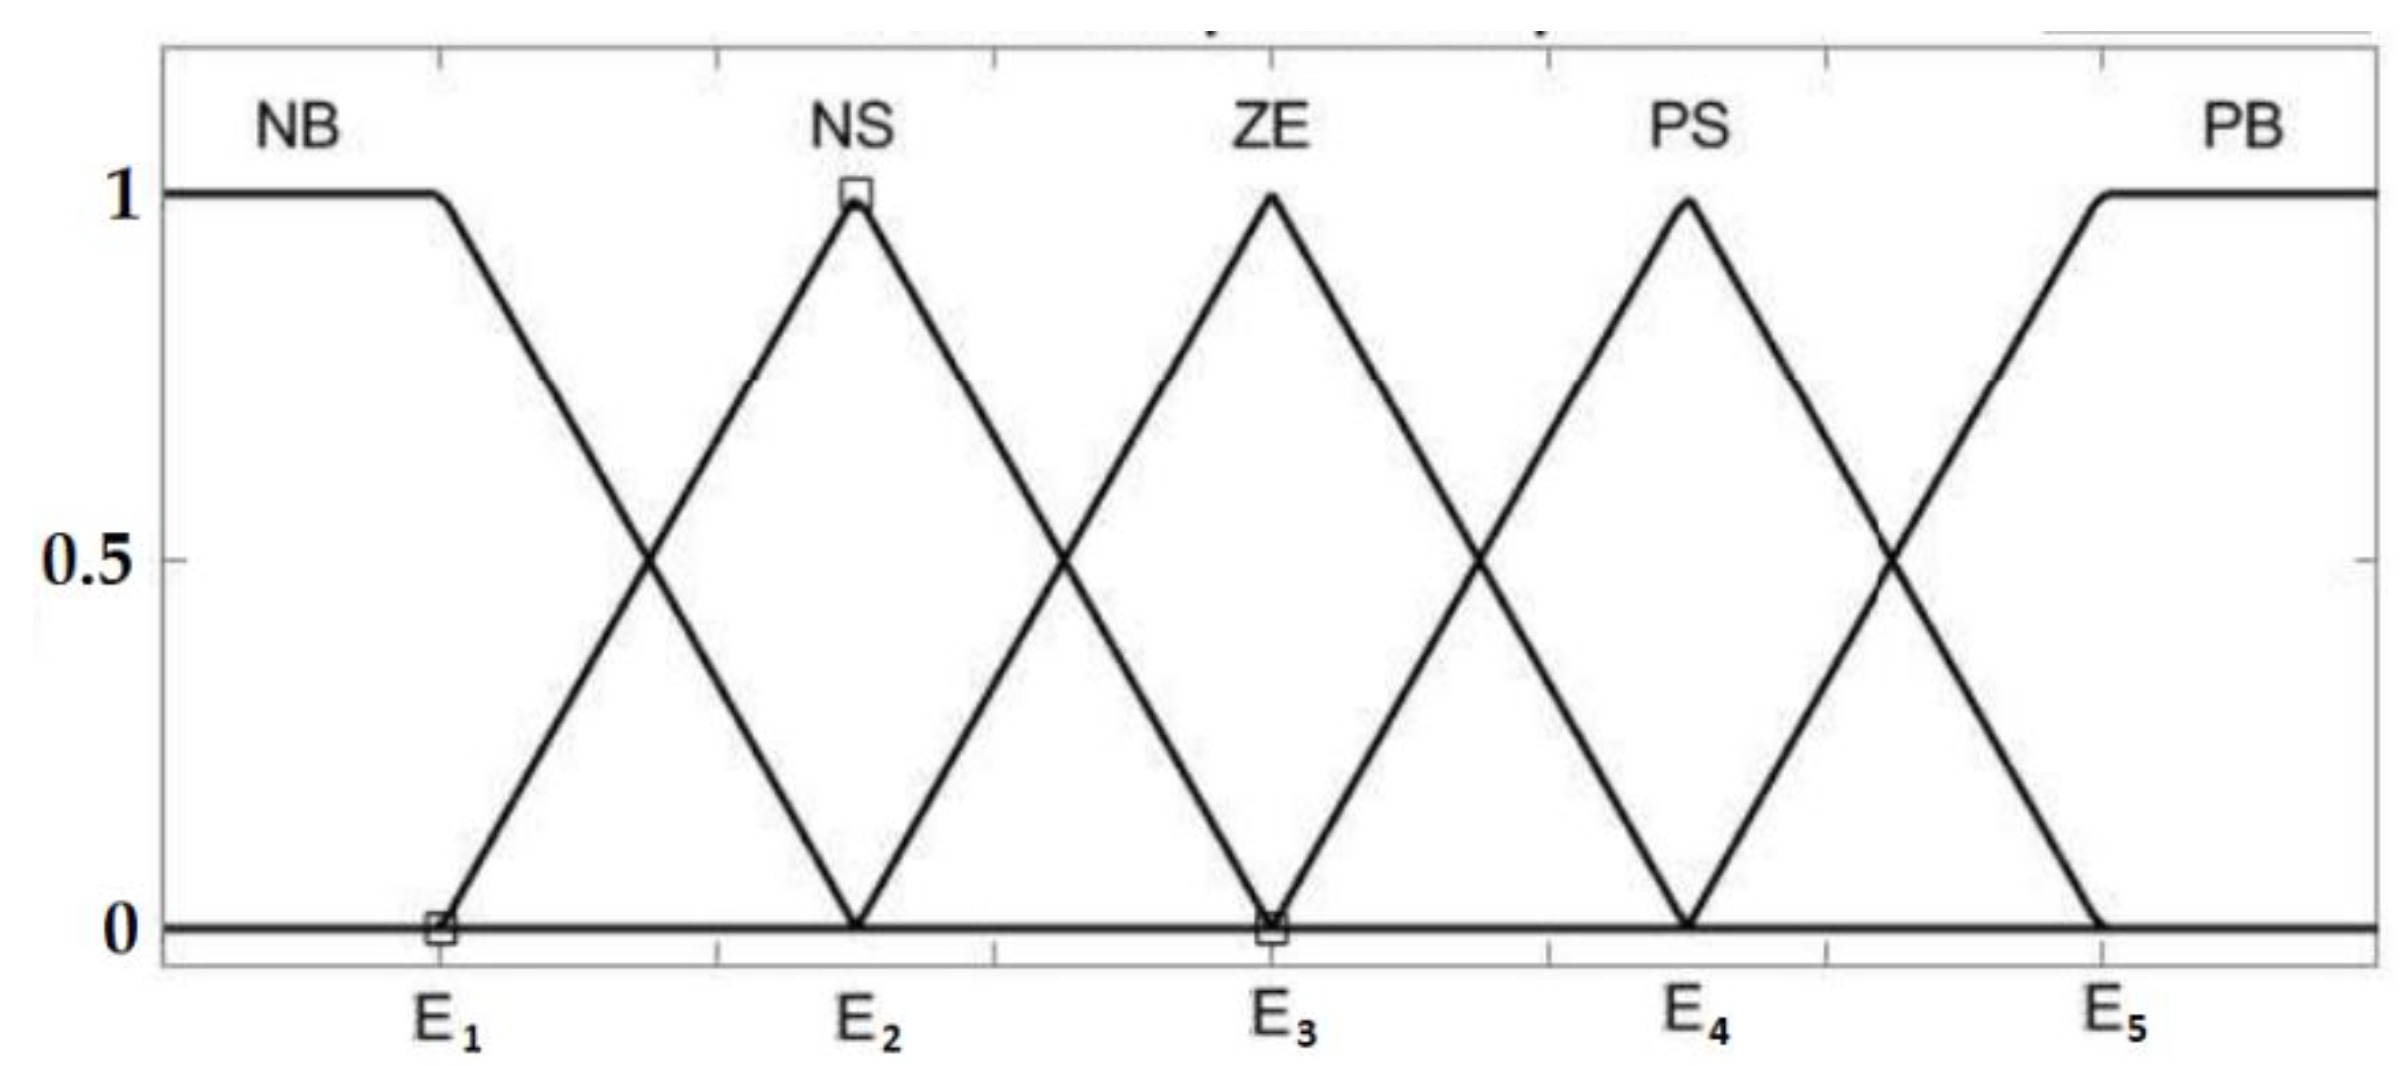
\includegraphics[width=0.85\textwidth]{_Bilder/BSP_Bild}
    \caption{Schematischer Aufbau von Zugehörigkeitsfunktionen eines Fuzzy-Reglers(übernommen aus \cite{Pehlivan2022}).}
    \label{fig:membership_funktionen_beispiel}
\end{figure}

Abbildung~\ref{fig:membership_funktionen_beispiel} zeigt schematisch den Aufbau von Zugehörigkeitsfunktionen eines Fuzzy-Reglers. Auch wenn hier beispielhaft andere Bezeichnungen verwendet werden, entspricht das dargestellte Prinzip dem im Projekt eingesetzten Regler.

\subsection{Reglerstruktur für x, y und theta}

Da sich ein omnidirektionaler Roboter unabhängig in x-Richtung, y-Richtung und um die eigene Achse $\theta$ bewegen kann, werden diese drei Bewegungsrichtungen getrennt geregelt. Für jede Richtung wird derselbe Fuzzy-Regler verwendet. Als Eingangsgrößen dienen jeweils der Positionsfehler sowie dessen Änderung. Im fortlaufenden beschrieben als error und derror. Für jede Richtung wird anhand des jeweiligen Positionsfehlers eine Sollgeschwindigkeit berechnet. Diese wird anschließend an die Kinematik übergeben und in Radgeschwindigkeiten umgerechnet. Die verwendeten Ein- und Ausgangsgrößen der drei Regelkanäle sind in Tabelle~\ref{tab:regelkanaele} dargestellt. \cite{Nguyen2022}

\begin{table}[H]
    \centering
    \caption{Ein- und Ausgangsgrößen der drei Regelkanäle}
    \label{tab:regelkanaele}
    \begin{tabular}{llll}
        \toprule
        Regelkanal & Eingänge & Ausgang & Physikalische Bedeutung \\
        \midrule
        x-Regler &
        $error_x$, $derror_x$ &
        $v_x$ &
        Geschwindigkeit in x-Richtung \\

        y-Regler &
        $error_y$, $derror_y$ &
        $v_y$ &
        Geschwindigkeit in y-Richtung \\

        $\theta$-Regler &
        $error_\theta$, $derror_\theta$ &
        $\omega$ &
        Drehgeschwindigkeit um die eigene Achse \\
        \bottomrule
    \end{tabular}
\end{table}

\subsection{Regelbasis}

Die Regelbasis legt fest, welche Stellgröße sich aus einer bestimmten Kombination von Fehler und Fehleränderung ergibt. Für jeden der drei Regelkanäle wird dieselbe $5 \times 5$-Regelmatrix verwendet. Die Zeilen beschreiben den aktuellen Fehlerzustand, die Spalten dessen Änderung. Das Ergebnis der Regelmatrix ist zunächst ein linguistischer Ausgangswert. Dieser wird anschließend in eine kontinuierliche numerische Stellgröße umgerechnet, welche direkt als Sollwert für die Bewegung des Roboters verwendet werden kann. Dieser Vorgang wird als Defuzzifizierung bezeichnet. Die verwendete Regelmatrix ist in Tabelle~\ref{tab:regelmatrix} dargestellt. \cite{Nguyen2022}

\begin{table}[H]
    \centering
    \caption{Regelmatrix des Fuzzy-Reglers}
    \label{tab:regelmatrix}
    \begin{tabular}{c|ccccc}
        \toprule
        $error \backslash derror$ & NB & NS & ZE & PS & PB \\
        \midrule
        NB & NB & NB & NB & NS & ZE \\
        NS & NB & NS & NS & ZE & PS \\
        ZE & NS & NS & ZE & PS & PS \\
        PS & NS & ZE & PS & PS & PB \\
        PB & ZE & PS & PB & PB & PB \\
        \bottomrule
    \end{tabular}
\end{table}

Die Matrix wurde so gewählt, dass bei großem Fehler zunächst eine starke Stellgröße erzeugt wird, während eine hohe Fehleränderung das Stellverhalten dämpft und dadurch ein weicheres Einfahren ermöglicht. Sie ist symmetrisch aufgebaut und sorgt dafür, dass große Fehler zu großen Stellgrößen führen, während Fehler nahe null nur kleine oder keine Stellgrößen erzeugen. Zusätzlich berücksichtigt der Regler die Fehleränderung. Zu Beginn einer Fahrt ist der Positionsfehler zwar groß, die Fehleränderung aufgrund der anfänglich geringen Geschwindigkeit jedoch noch klein. Dadurch wird zunächst keine maximale Stellgröße ausgegeben, sondern der Roboter beschleunigt kontrolliert und ruckarm. Bewegt sich der Roboter bereits in Richtung des Zieles und der Fehler nimmt kontinuierlich ab, reduziert die Regelbasis die Stellgröße frühzeitig. Dadurch wird ein Überschwingen vermieden und ein gleichmäßiges sowie ruhiges Einfahren in die Zielposition erreicht.

\subsection{Skalierung der realen Größen}

Der Fuzzy-Regler arbeitet ausschließlich mit normierten Ein- und Ausgangsgrößen im Wertebereich von $-1$ bis $+1$. Reale Positions- und Winkelfehler können jedoch deutlich größere Werte annehmen und müssen daher vor der Verarbeitung auf diesen Bereich abgebildet werden. Ebenso muss die vom Fuzzy-Regler berechnete normierte Stellgröße anschließend wieder in reale translatorische beziehungsweise rotatorische Geschwindigkeiten umgerechnet werden. Die Skalierung erfolgt über jeweils einen Faktor für die Eingangs- und Ausgangsgrößen. Die Eingangsskalierung bestimmt, welcher reale Fehler einer maximalen Fuzzy-Eingangsgröße entspricht. Eine hohe Skalierung führt dazu, dass bereits kleine Fehler als große Fuzzy-Fehler interpretiert werden, wodurch der Regler aggressiver reagiert. Eine kleinere Skalierung bewirkt dagegen ein ruhigeres Regelverhalten. Die Ausgangsskalierung legt fest, welche reale Geschwindigkeit einer maximalen Fuzzy-Stellgröße entspricht und beeinflusst damit unmittelbar die Dynamik des Roboters. Für die translatorischen Bewegungen in x- und y-Richtung sowie für die Rotation wurden getrennte Skalierungsparameter verwendet, da sich die erforderlichen Stellgrößen und Regelcharakteristiken deutlich unterscheiden. Die Bestimmung geeigneter Skalierungsparameter erfolgt in Kapitel~\ref{sec:simulation} mithilfe einer simulationsbasierten Optimierung.

\section{Parameterbestimmung durch Python-Simulation}
\label{sec:simulation}

Ziel der Simulation war nicht die Bestimmung vollständig optimaler Reglerparameter, sondern die Ermittlung geeigneter Ausgangswerte für die anschließende Feinabstimmung am realen Roboter. Hierzu wurde eine Simulationsumgebung entwickelt, welche das Regelverhalten des Roboters reproduziert und unterschiedliche Parametersätze anhand einer Kostenfunktion bewertet. Optimiert wurden ausschließlich die sechs Skalierungsparameter des Fuzzy-Reglers. Diese bestimmen die Abbildung zwischen realen Positions- und Winkelfehlern sowie dem normierten Fuzzy-Bereich und legen gleichzeitig fest, wie die berechneten Stellgrößen wieder in reale translatorische und rotatorische Geschwindigkeiten umgesetzt werden.

\subsection{Zentrale Konfiguration}

Alle wesentlichen Einstellungen der Simulation wurden in einer zentralen \texttt{CONFIG}-Struktur zusammengefasst. Dadurch können Start- und Zielposition, Simulationsparameter, Robotergeometrie, Kostenfunktionsgewichte sowie Optimierungsparameter an einer Stelle angepasst werden. Dies erleichtert das Testen verschiedener Einstellungen und verbessert gleichzeitig die Übersichtlichkeit des Programms.
Diese eizelnen Teile der \texttt{CONFIG}-Struktur sind zur Übersicht nochmals in Tabelle~\ref{tab:config} veranschaulicht.

\begin{table}[H]
    \centering
    \caption{Zentrale Konfiguration der Simulation}
    \label{tab:config}
    \small
    \begin{tabularx}{\textwidth}{lXX}
        \toprule
        \textbf{Bereich} & \textbf{Wichtige Parameter} & \textbf{Bedeutung} \\
        \midrule

        \texttt{start\_params} &
        \texttt{error\_scale\_xy}, \texttt{derror\_scale\_xy},
        \texttt{output\_scale\_xy}, \texttt{error\_scale\_theta},
        \texttt{derror\_scale\_theta},
        \texttt{output\_scale\_theta} &
        Startwerte der zu optimierenden Reglerparameter \\

        \texttt{pose} &
        \texttt{x\_start}, \texttt{y\_start},
        \texttt{theta\_start},
        \texttt{x\_target}, \texttt{y\_target},
        \texttt{theta\_target} &
        Start- und Zielposition der Simulation \\

        \texttt{simulation} &
        \texttt{dt}, \texttt{steps},
        \texttt{v\_limit}, \texttt{omega\_limit},
        \texttt{pos\_tol},
        \texttt{theta\_tol} &
        Zeitschritt, Simulationsdauer und Abbruchbedingungen \\

        \texttt{robot} &
        \texttt{robot\_radius},
        \texttt{wheel\_diameter},
        \texttt{wheel\_linear\_limit},
        \texttt{wheel\_angles\_deg} &
        Geometrie und Begrenzungen des omnidirektionalen Roboters \\

        \texttt{cost\_weights} &
        \texttt{pos\_weight},
        \texttt{theta\_weight},
        \texttt{time\_weight},
        \texttt{smooth\_*} &
        Gewichtung der Kostenfunktion \\

        \texttt{optimization} &
        \texttt{maxiter},
        \texttt{popsize},
        \texttt{tol},
        \texttt{seed},
        \texttt{polish} &
        Einstellungen des Optimierers \\

        \bottomrule
    \end{tabularx}
\end{table}

\subsection{Skalierung}

Für die Simulation wurden die in Kapitel~\ref{sec:simulation} beschriebenen Skalierungsparameter verwendet. Die Positionsfehler werden zunächst auf einen Bereich von \SI{-1}{\meter} bis \SI{1}{\meter} normiert und anschließend mithilfe der Skalierungsparameter auf den Fuzzy-Eingangsbereich abgebildet. Für den Winkelfehler erfolgt dieselbe Vorgehensweise mit einem Bereich von $-\pi$ bis $+\pi$. Zur Einhaltung der physikalischen Grenzen werden die Sollgeschwindigkeiten zusätzlich begrenzt. Für die translatorische Bewegung wurde eine maximale Geschwindigkeit von \SI{0.94}{\meter\per\second} verwendet. Die maximal zulässige Winkelgeschwindigkeit ergibt sich aus der maximalen Umfangsgeschwindigkeit der Räder und dem Abstand der Räder zum Mittelpunkt des Roboters:

\begin{equation}
    v_{\mathrm{Rad}} = r \cdot \omega
    \label{eq:radgeschwindigkeit}
\end{equation}

Daraus folgt:

\begin{equation}
    \omega_{\mathrm{max}}
    =
    \frac{v_{\mathrm{Rad,max}}}{r}
    =
    \frac{\SI{0.94}{\meter\per\second}}{\SI{0.15}{\meter}}
    \approx
    \SI{6.27}{\radian\per\second}.
    \label{eq:omega_max}
\end{equation}

Diese Werte dienen als obere Begrenzung der Sollgeschwindigkeiten innerhalb der Simulation und stellen sicher, dass keine physikalisch nicht realisierbaren Stellgrößen erzeugt werden.

\subsection{Simulationsmodell und Ablauf}

Die Simulation bildet den vollständigen Regelkreis des Roboters nach und dient als Grundlage für die Bewertung unterschiedlicher Parametersätze. Hierzu werden drei Instanzen des in Kapitel~2 ODERSO beschriebenen Fuzzy-Reglers für die Bewegungen in x-Richtung, y-Richtung sowie für die Orientierung verwendet. Zu Beginn jedes Simulationsschritts werden aus der aktuellen Positions- und Winkelfehler sowie deren Änderungen bestimmt. Diese Größen werden dem Fuzzy-Regler übergeben, welcher daraus translatorische und rotatorische Sollgeschwindigkeiten berechnet. Anschließend werden die Sollgeschwindigkeiten mithilfe der inversen Kinematik in Radgeschwindigkeiten umgerechnet. Überschreiten diese die zulässigen Grenzwerte des Roboters, erfolgt eine Begrenzung auf die maximal realisierbaren Radgeschwindigkeiten. Aus den begrenzten Radgeschwindigkeiten werden anschließend über die Vorwärtskinematik die tatsächlich erreichbaren translatorischen und rotatorischen Geschwindigkeiten bestimmt. Mit diesen Geschwindigkeiten wird die Roboterpose für den nächsten Simulationsschritt berechnet. Dieser Ablauf wird solange wiederholt, bis die Zielpose innerhalb der vorgegebenen Positions- und Orientierungstoleranzen erreicht ist oder die maximale Simulationsdauer überschritten wird.

\subsection{Kostenfunktion}

Die Qualität eines Parametersatzes wird über eine Kostenfunktion bewertet. Dabei werden sowohl die Genauigkeit der Zielerreichung als auch das dynamische Verhalten des Roboters berücksichtigt. Die Gesamtkosten setzen sich aus Positions-, Winkel-, Zeit-, Stellgrößen- und Glattheitskosten sowie einem Strafterm zusammen. Die einzelnen Bestandteile der Kostenfunktion sind in Tabelle~\ref{tab:kostenfunktion} zusammengefasst.

\begin{table}[H]
    \centering
    \caption{Bestandteile der Kostenfunktion}
    \label{tab:kostenfunktion}
    \small
    \begin{tabularx}{\textwidth}{l l X}
        \toprule
        \textbf{Kostenanteil} & \textbf{Term} & \textbf{Bedeutung} \\
        \midrule
        Positionskosten &
        $J_{\mathrm{pos}}$ &
        Bewerten die verbleibende Positionsabweichung am Ende der Simulation. \\

        Winkelkosten &
        $J_{\theta}$ &
        Bewerten die verbleibende Orientierungsabweichung. \\

        Zeitkosten &
        $J_t$ &
        Bevorzugen kurze Fahrzeiten beziehungsweise wenige Simulationsschritte. \\

        Stellgrößenkosten &
        $J_u$ &
        Bestrafen hohe translatorische und rotatorische Stellgrößen. \\

        Glattheitskosten &
        $J_s$ &
        Bestrafen Änderungen der Stellgrößen und reduzieren dadurch Oszillationen. \\

        Penalty &
        $J_{\mathrm{penalty}}$ &
        Zusatzkosten, wenn das Ziel innerhalb der vorgegebenen Toleranzen nicht erreicht wird. \\
        \bottomrule
    \end{tabularx}
\end{table}

Die Gewichtung der einzelnen Kostenanteile wurde anhand mehrerer Simulationsläufe iterativ abgestimmt. Ziel war es, ein ausgewogenes Optimierungsverhalten hinsichtlich der Zielgenauigkeit, der Fahrzeit sowie eines möglichst ruhigen und kontinuierlichen Stellgrößenverlaufs zu erzielen. Daraus ergibt sich die folgende Gesamtkostenfunktion:

\begin{equation}
\begin{aligned}
J ={}&
0.8\,J_{\mathrm{pos}}
+10.0\,J_{\theta}
+0.001\,J_t \\
&+J_u
+J_s
+J_{\mathrm{penalty}} .
\end{aligned}
\label{eq:kostenfunktion}
\end{equation}

Die Stellgrößenkosten ($J_u$) berücksichtigen unterschiedliche Gewichtungen für translatorische und rotatorische Stellgrößen. Analog werden in den Glattheitskosten ($J_s$) Änderungen der translatorischen und rotatorischen Stellgrößen unterschiedlich gewichtet, um einen möglichst ruhigen und kontinuierlichen Stellgrößenverlauf zu fördern. Der Strafterm ($J_{\mathrm{penalty}}$) nimmt den Wert 50 an, wenn das Ziel innerhalb der vorgegebenen Toleranzen nicht erreicht wird; andernfalls ist ($J_{\mathrm{penalty}}=0$).


\subsection{Optimierungsverfahren}

Zur Optimierung der sechs Skalierungsparameter wurde das Verfahren \texttt{differential\_evolution} aus der Bibliothek \texttt{scipy.optimize} verwendet. Aufgrund seiner Robustheit und der guten Dokumentation wurde es für diese Arbeit ausgewählt.

\subsection{Modellannahmen und Einschränkungen}

Zur Begrenzung des Rechenaufwands wurden bei der Simulation bewusst mehrere Vereinfachungen vorgenommen.Das Robotermodell berücksichtigt ausschließlich die Kinematik des Fahrzeugs. Dynamische Effekte wie Massenträgheiten, Reibung, Radschlupf oder das Verhalten der Motoren werden nicht modelliert. Eine dynamische Modellierung erhöht die Genauigkeit stärker bei hohen Geschwindigkeiten und Beschleunigungen. Da die Optimierung jedoch lediglich geeignete Startparameter für die anschließende Feinabstimmung liefern sollte und die höchste Genauigkeit vor allem beim langsamen Anfahren der Zielposition erforderlich ist, wurde diese Vereinfachung als sinnvoll angesehen. Darüber hinaus wurden ausschließlich die sechs Skalierungsparameter optimiert. Die Regelbasis sowie die Membership-Funktionen blieben unverändert, da deren zusätzliche Optimierung  die Rechenzeit deutlich erhöht hätte. Außerdem erfolgte die Optimierung anhand einer einzelnen Referenzfahrt. Eine Bewertung über verschiedene Fahrprofile hätte robustere Parametersätze geliefert, den Rechenaufwand jedoch nahezu proportional zur Anzahl der zusätzlichen Simulationen erhöht. Bereits unter diesen Randbedingungen betrug die Rechenzeit der Optimierung mehr als sieben Stunden. Die getroffenen Vereinfachungen stellen daher einen sinnvollen Kompromiss zwischen Modellgenauigkeit und Rechenaufwand dar. \cite{Mondal2019,Mendili2017}

\subsection{Ergebnis der Simulation}

Die Simulation mit den Startparametern erreicht das Ziel bereits, zeigt aber eine höhere Gesamtkostenbewertung als der optimierte Parametersatz. Abbildung~\ref{fig:simulation_gesamtauswertung} zeigt die Membership-Funktionen, Trajektorie, Winkelverlauf, Positions- und Geschindigkeisverläufe der simulierten Fahrt mit den Startwerten und der optimierten Fahrt.

\begin{figure}[H]
    \centering
     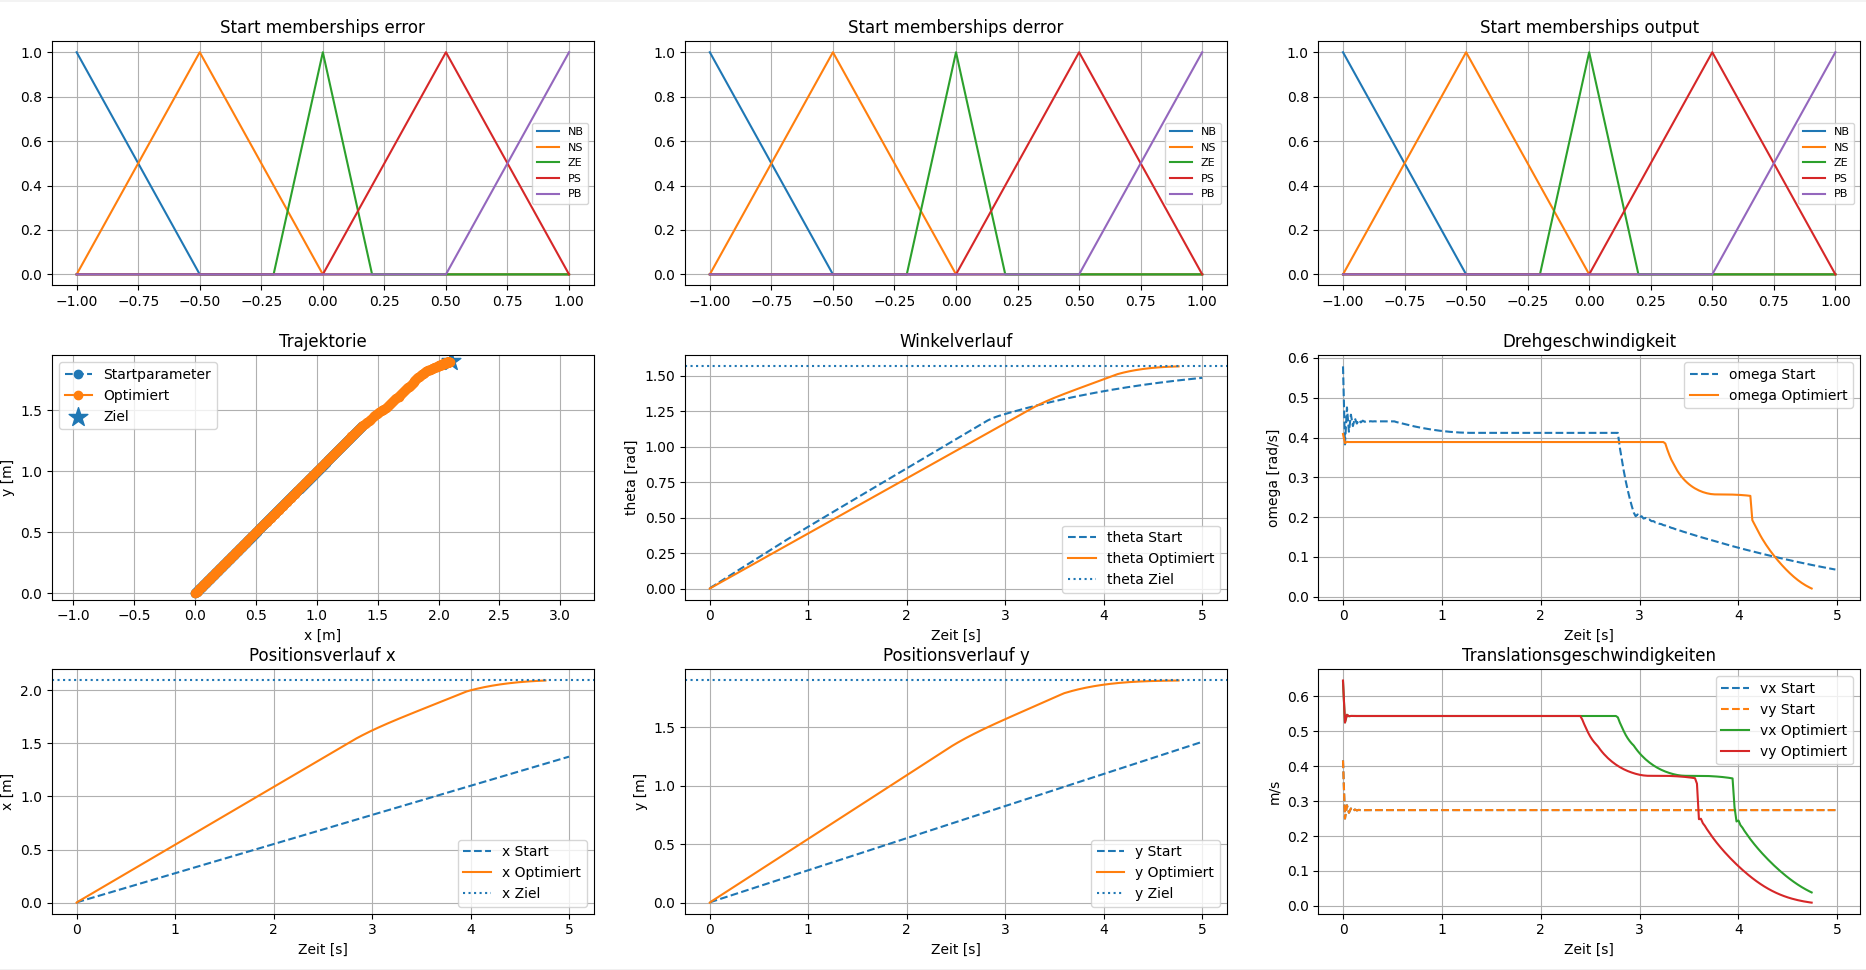
\includegraphics[width=\textwidth]{_Bilder/simulation_gesamtauswertung}
    \caption{Gesamtauswertung der Simulation mit Membership-Funktionen, Trajektorie, Winkelverlauf, Positions- und Geschindigkeisverläufen.}
    \label{fig:simulation_gesamtauswertung}
\end{figure}

\subsection{Numerische Ergebnisse}

Die Ergebnisse wurden per Konsolenausgabe dokumentiert und umfassen die Kosten, Endwerte und optimierten Parameter. Für die Startparameter ergibt sich eine Gesamtkostenbewertung von etwa $661{,}529552$. Nach der Optimierung sinken die Kosten auf etwa $22{,}89056$. 
Die ermittelten Werte im Vergleich zu den gesetzten Simulationsstartwerten sind in Tabelle~\ref{tab:optimierte_parameter} dargestellt.




\begin{table}[H]
    \centering
    \caption{Vergleich der Startparameter und optimierten Skalierungsparameter}
    \label{tab:optimierte_parameter}
    \small
    \begin{tabularx}{\textwidth}{l c c X}
        \toprule
        \textbf{Parameter} & \textbf{Start} & \textbf{Optimiert} & \textbf{Interpretation} \\
        \midrule

        \texttt{error\_scale\_xy} &
        $2{,}000000$ &
        $1{,}697825$ &
        Positionsfehler in x/y werden im Fuzzy-Bereich stärker gewichtet. \\

        \texttt{derror\_scale\_xy} &
        $0{,}500000$ &
        $0{,}121643$  &
        Fehleränderungen in x/y werden etwas schwächer gewichtet. \\

        \texttt{output\_scale\_xy} &
        $0{,}500000$ &
        $0{,}780699$ &
        Maximale translatorische Ausgangsgeschwindigkeit wird reduziert. \\

        \texttt{error\_scale\_theta} &
        $1{,}500000$ &
        $3{,}277952$ &
        Winkelfehler wird deutlich empfindlicher bewertet. \\

        \texttt{derror\_scale\_theta} &
        $0{,}300000$ &
        $0{,}123418$ &
        Änderung des Winkelfehlers wird leicht schwächer gewichtet. \\

        \texttt{output\_scale\_theta} &
        $1{,}000000$ &
        $0{,}530832$ &
        Drehgeschwindigkeit wird etwa halbiert. \\

        \bottomrule
    \end{tabularx}
\end{table}

\subsection{Interpretation der optimierten Skalierung}

Die optimierte Skalierung zeigt unterschiedliche Anpassungen der Ein- und Ausgangsgrößen. Für den Positionsregler werden die Eingangsskalierungen \texttt{error\_xy} und \texttt{derror\_xy} reduziert, während die Ausgangsskalierung \texttt{output\_xy} erhöht wird. Dadurch reagiert der Regler weniger empfindlich auf Positionsfehler, gleichzeitig werden die resultierenden Fuzzy-Ausgangswerte stärker in Translationsgeschwindigkeit umgesetzt.

Für die Winkelregelung wird \texttt{error\_theta} steiler skaliert und erreicht den Sättigungsbereich bereits bei kleineren Winkelabweichungen. Gleichzeitig werden \texttt{derror\_theta} und \texttt{output\_theta} reduziert, wodurch die maximale Drehgeschwindigkeit begrenzt und ein ruhigeres Regelverhalten erzielt wird. Abbildung~\ref{fig:skalierung_start_optimiert} verdeutlicht diese Anpassungen.

\begin{figure}[H]
    \centering
     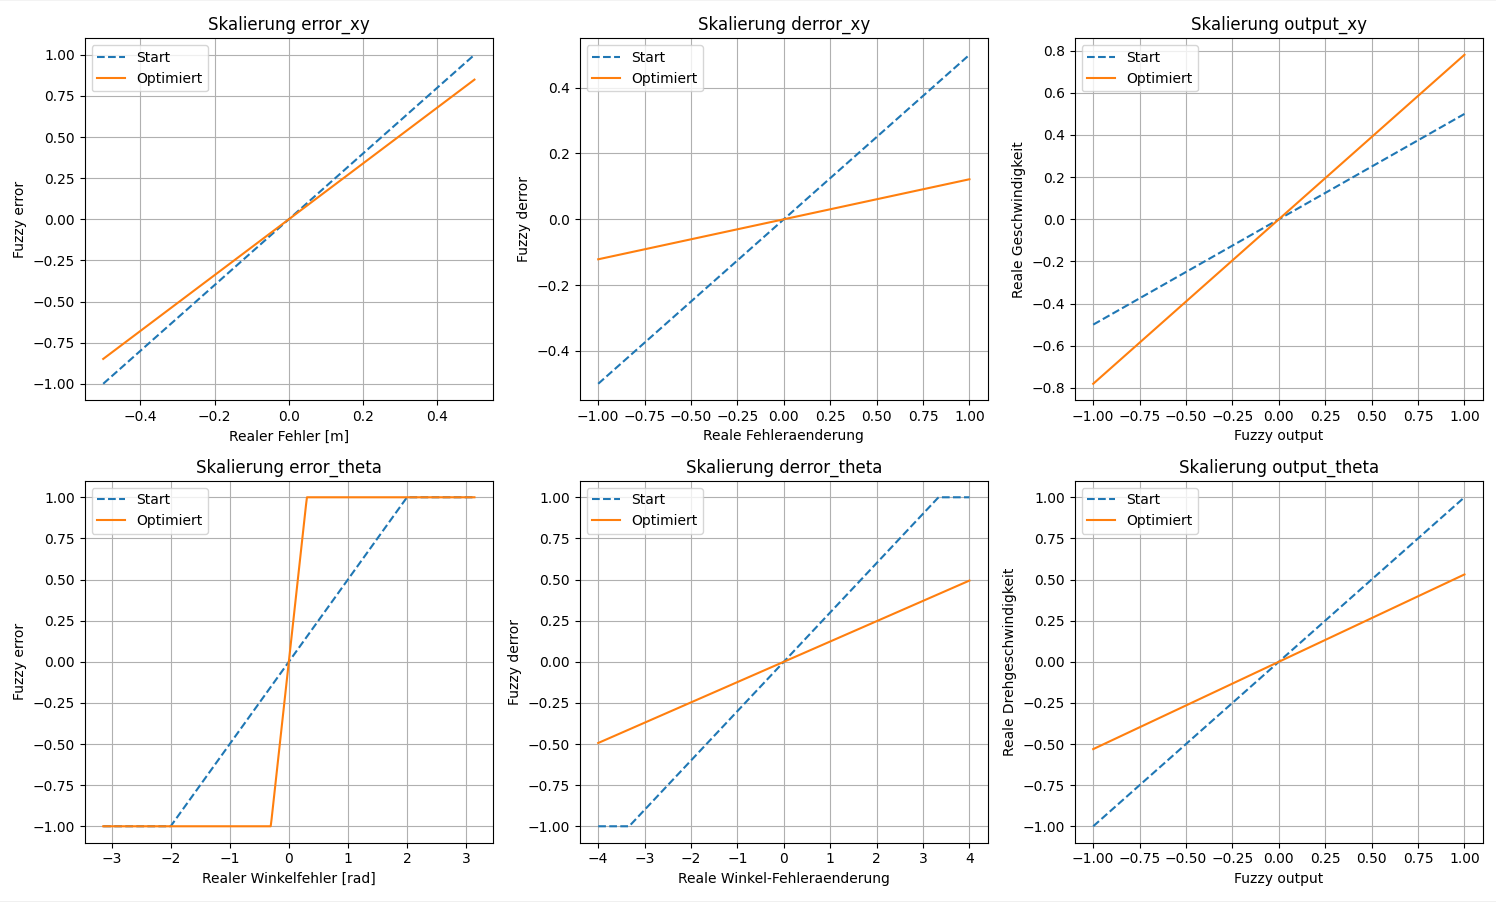
\includegraphics[width=\textwidth]{_Bilder/skalierung_start_optimiert}
    \caption{Vergleich der Start- und Endskalierungen für Positionsfehler, Fehleränderung und Ausgangsgrößen.}
    \label{fig:skalierung_start_optimiert}
\end{figure}

\subsection{Bewertung der Simulation}

Die Simulation liefert einen strukturierten ersten Parametersatz und zeigt, dass der Regler grundsätzlich funktioniert. Gleichzeitig ist sie bewusst einfach gehalten. Sie enthält keine vollständige Modellierung von Haft- und Gleitreibung, Radschlupf, Motorverzögerungen, Kommunikationslatenzen oder Messrauschens. Deshalb darf das Simulationsergebnis nicht direkt als endgültige Parametrierung verstanden werden. Es ist vielmehr ein Startpunkt für die reale Anpassung. Besonders kritisch ist der Unterschied zwischen idealer Kinematik und realer Fahrmechanik. In der Simulation wird angenommen, dass die berechneten Radgeschwindigkeiten direkt umgesetzt werden. 

\section{Umsetzung des Fuzzy-Reglers in der Robotersteuerung}

\subsection{Integration in die bestehende Steuerungsstruktur}

Der in Kapitel~3 entwickelte Fuzzy-Regler wurde in die bestehende Robotersteuerung unter TwinCAT integriert. Dabei ersetzt er ausschließlich die Berechnung der Sollgeschwindigkeiten innerhalb der Positionsregelung. Die darunterliegende Geschwindigkeitsregelung der einzelnen Motoren sowie die inverse Kinematik bleiben unverändert bestehen. Die zentrale Ablaufsteuerung erfolgt innerhalb der \texttt{MainMotorTask}. Dort werden die aktuelle Roboterpsition sowie die Sollposition eingelesen und an den Funktionsbaustein \texttt{FB\_Positionsregler} übergeben. Dieser berechnet aus den aktuellen Roboter- und Sollwerten die translatorischen Sollgeschwindigkeiten in x- und y-Richtung sowie die rotatorische Sollgeschwindigkeit. Da diese Geschwindigkeiten zunächst im Weltkoordinatensystem vorliegen, werden sie anschließend in das Roboterkoordinatensystem transformiert und an die inverse Kinematik übergeben. Dort werden die Sollgeschwindigkeiten der einzelnen Räder berechnet und als Führungsgrößen an die bestehenden Geschwindigkeitsregler der Motoren weitergegeben. Durch diese Struktur beschränkten sich die Änderungen an der Software auf den Bereich der Positionsregelung. Die vorhandene Motorregelung sowie die Hardwareansteuerung konnten unverändert übernommen werden, wodurch sich der Fuzzy-Regler ohne grundlegende Änderungen in die bestehende Softwarearchitektur integrieren ließ.

\subsection{Praktische Erweiterungen}

Bei der Übertragung des simulierten Fuzzy-Reglers auf den realen Roboter zeigte sich, dass zusätzliche Maßnahmen erforderlich sind, um unter realen Einsatzbedingungen ein stabiles und robustes Regelverhalten sicherzustellen. Hierzu wurden insbesondere die Zielerkennung erweitert sowie die Verarbeitung der Kameradaten angepasst. Zur sicheren Erkennung der Zielposition wurde im \texttt{FB\_Positionsregler} eine Hysterese implementiert. Ohne diese würde der Roboter bereits bei kleinsten Positionsänderungen oder Messabweichungen fortlaufend zwischen den Zuständen \glqq Ziel erreicht\grqq{} und \glqq Ziel nicht erreicht\grqq{} wechseln und dadurch unnötige Korrekturbewegungen ausführen. Durch unterschiedliche Schwellwerte für das Erreichen und Verlassen des Zielbereichs verbleibt der Roboter innerhalb einer definierten Toleranz stabil im Endzustand. Eine weitere Anpassung betrifft die Verarbeitung der Kameramessungen. Die Zykluszeit der Robotersteuerung ist deutlich kleiner als die Aktualisierungsrate der Kamera, sodass derselbe Messwert häufig über mehrere Regelzyklen hinweg anliegt. Würde dieser in jedem Zyklus erneut verarbeitet, ergäbe sich über mehrere Zyklen hinweg keine Fehleränderung. Beim Eintreffen einer neuen Kameramessung entstünde dadurch eine sprunghafte Änderung, welche das Regelverhalten negativ beeinflussen könnte. Aus diesem Grund wird zunächst geprüft, ob tatsächlich eine neue Kameramessung vorliegt. Nur in diesem Fall wird die Fehleränderung aktualisiert. Liegt kein neuer Kamerawert vor, wird die Roboterpose mithilfe der Motordaten fortgeschrieben. Befindet sich der Roboter bereits innerhalb des Zielbereichs, bleibt dieser Zustand unabhängig davon erhalten, sodass die Zielposition weiterhin zuverlässig erkannt wird. Durch diese Ergänzungen konnte der in der Simulation entwickelte Regler erfolgreich auf das reale System übertragen werden. Insbesondere die Hysterese sowie die angepasste Verarbeitung der Kameradaten tragen zu einem ruhigen und stabilen Fahrverhalten des Roboters bei.

\section{Test am realen System, Ergebnisse und Erkenntnisse}

Nach der simulationsbasierten Parametrierung wurde das Regelverhalten am realen System untersucht. Zunächst wurde die grundsätzliche Funktion des Fuzzy-Reglers anhand einfacher Fahrmanöver überprüft, um die korrekte Integration in die Robotersteuerung sicherzustellen. Anschließend erfolgte die Erprobung unter realen Einsatzbedingungen. Hierbei wurden verschiedene Zielpositionen und Orientierungen angefahren und das Fahrverhalten hinsichtlich bewertet. Besonderes Augenmerk lag dabei auf einem ruhigen Anfahrverhalten, dem Vermeiden von Überschwingen sowie einem gleichmäßigen und stabilen Einfahren in die Zielposition. Während der Versuche wurden die Daten der drei Antriebsmotoren aufgezeichnet. Mithilfe der Vorwärtskinematik wurde aus diesen Messdaten die tatsächlich zurückgelegte Trajektorie des Roboters rekonstruiert und anschließend grafisch dargestellt. Die Auswertung dieser Fahrten diente sowohl der Beurteilung der Regelgüte als auch der Feinabstimmung der zuvor in der Simulation ermittelten Reglerparameter.

\subsection{Positionsfahrt im realen System}

Zur Überprüfung der Positionsregelung wurde eine beispielhafte Fahrt mit mehreren Zielpositionen durchgeführt. Ausgehend von einer beliebigen Startposition wurden vier Zielpunkte im Arbeitsraum angefahren. Zwischen den einzelnen Zielpunkten wurden sowohl translatorische Bewegungen als auch Änderungen der Roboterorientierung durchgeführt. Am zweiten Zielpunkt wurde ausschließlich die Sollorientierung geändert, während die Position unverändert blieb.  Abbildung~\ref{fig:reale_positionsfahrt_xy} zeigt die rekonstruierte Trajektorie des Roboters in der XY-Ebene. Die schwarze Linie stellt die berechnete Fahrbahn dar, während die roten Kreuze die vorgegebenen Zielpositionen markieren. Zusätzlich sind die Sollorientierungen an den einzelnen Zielpunkten sowie die während der Fahrt gemessene Orientierung des Roboters durch blaue Pfeile dargestellt.

\begin{figure}[H]
    \centering
     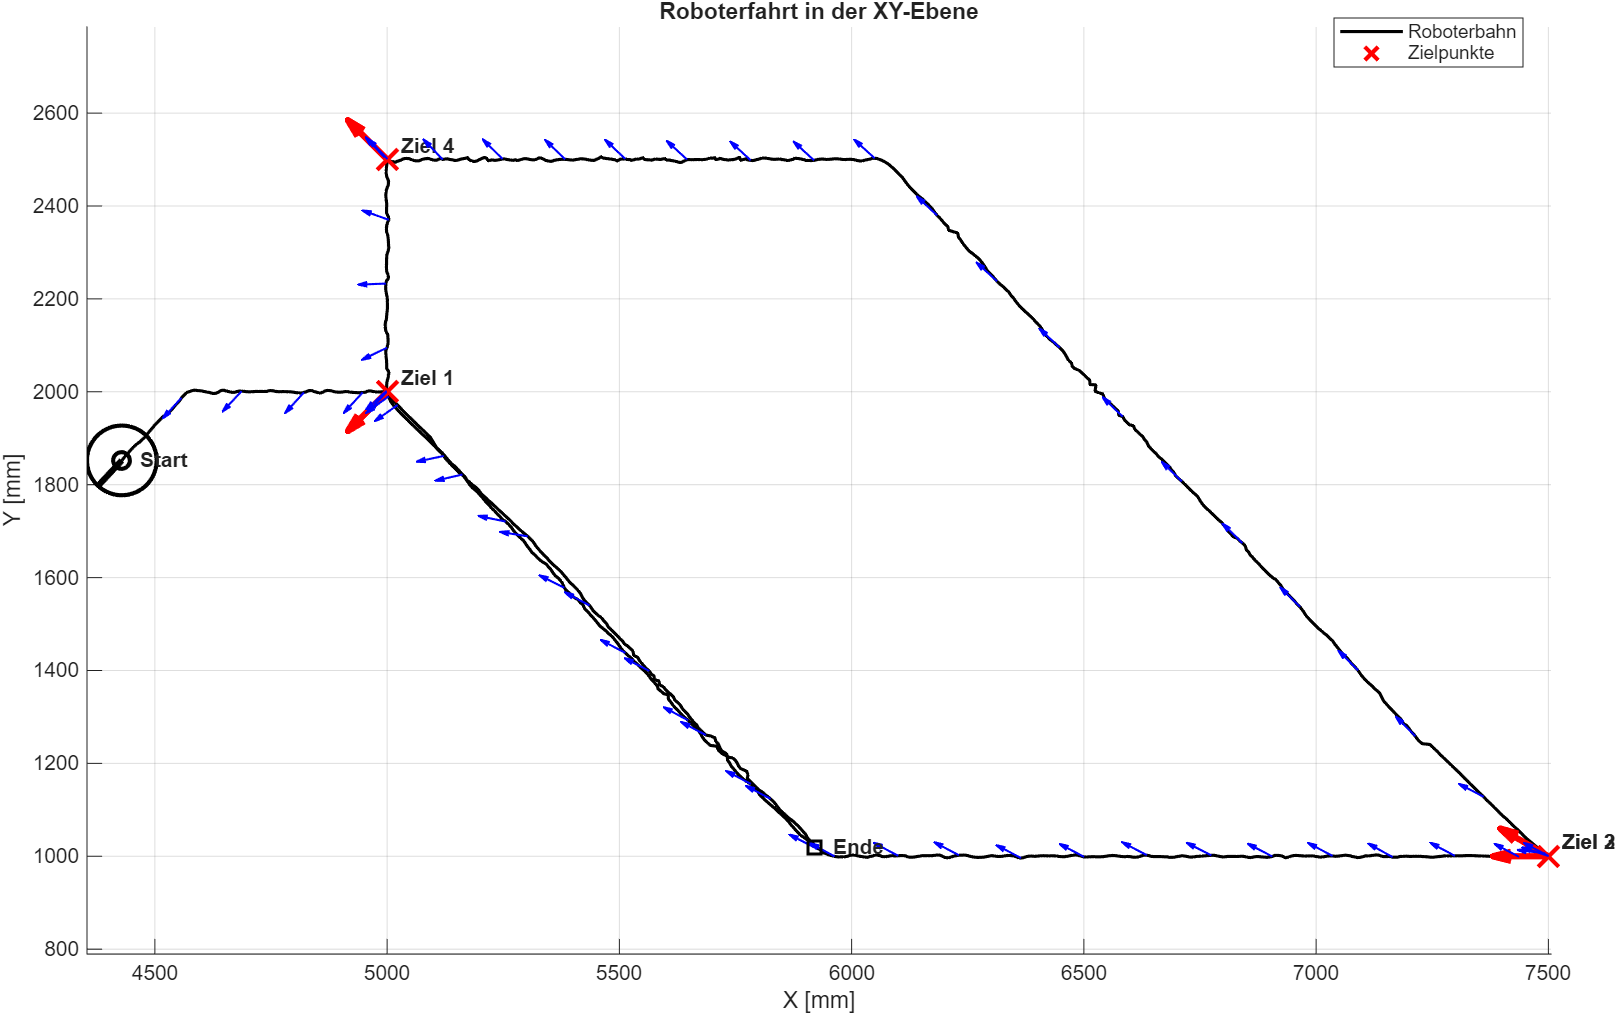
\includegraphics[width=0.95\textwidth]{_Bilder/reale_positionsfahrt_xy}
    \caption{Rekonstruierte Roboterfahrt in der XY-Ebene mit Start, Ende und Zielpunkten.}
    \label{fig:reale_positionsfahrt_xy}
\end{figure}

Die Messergebnisse zeigen, dass alle Zielpositionen zuverlässig erreicht werden. Auch die Orientierungsänderungen werden während der Fahrt korrekt ausgeführt. Die rekonstruierten Fahrbahnen verlaufen weitgehend entlang der geplanten Bewegungsrichtungen und bestätigen die korrekte Umsetzung des Fuzzy-Reglers auf dem realen System. Zur besseren Veranschaulichung der einzelnen Bewegungsabschnitte ist in Abbildung~\ref{fig:reale_positionsfahrt_y} exemplarisch der Verlauf der y-Position über der Zeit dargestellt. Die einzelnen Plateaus entsprechen den angefahrenen Zielpositionen, während die linearen Übergänge die Bewegungen zwischen den einzelnen Punkten zeigen. Die Abbildung verdeutlicht, dass die Zielpositionen stabil erreicht werden und verhart bis die anderen Position, z.B. in X-Richtung, erreicht sind. 

\begin{figure}[H]
    \centering
    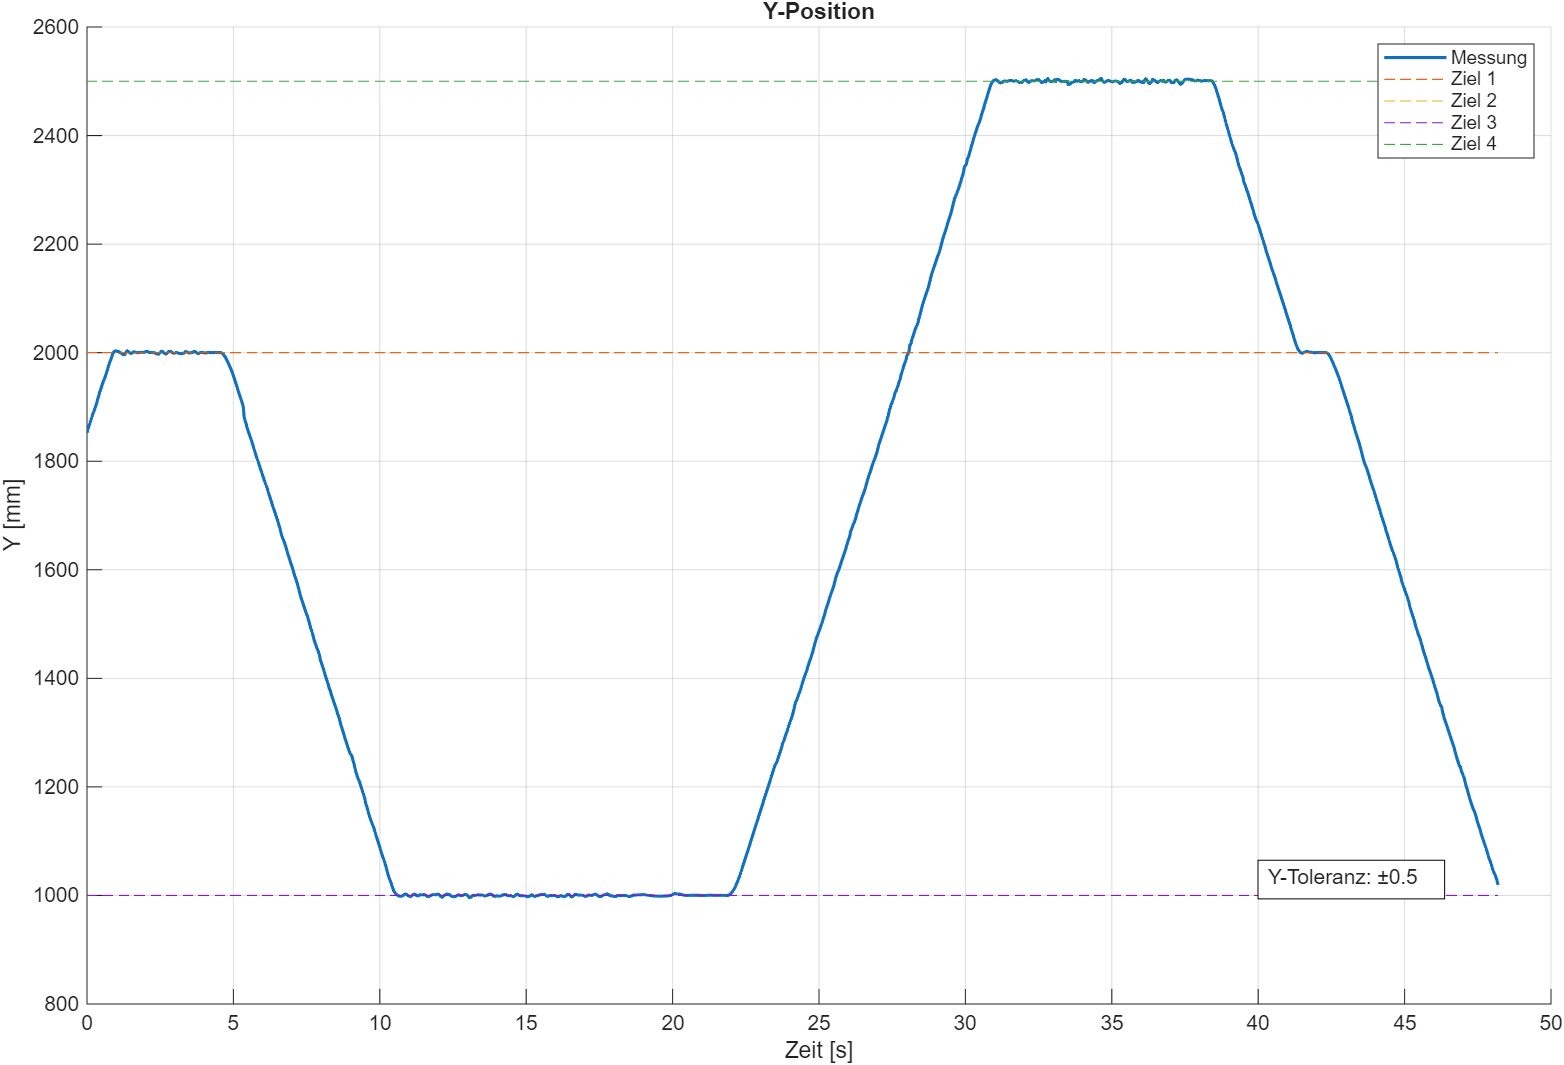
\includegraphics[width=0.9\textwidth]{_Bilder/reale_positionsfahrt_y}
    \caption{Rekonstruierte Roboterfahrt in der y-Richtung.}
    \label{fig:reale_positionsfahrt_y}
\end{figure}

\subsection{Anfahrt des Ablagepunkts}

Nach der grundsätzlichen Verifikation der Positionsregelung wurde das Verhalten des Roboters an einem für den praktischen Einsatz besonders relevanten Ablagepunkt untersucht. Für diesen Zielpunkt galten deutlich engere Positions- und Orientierungstoleranzen, da ein präzises Anfahren erforderlich ist, um einen sicheren Ablagevorgang zu gewährleisten. Wie bereits im vorherigen Versuch wurden während der Fahrt die Drehgeberdaten der drei Antriebsmotoren aufgezeichnet und mithilfe der Vorwärtskinematik die tatsächlich zurückgelegte Trajektorie rekonstruiert. Ziel 2 stellt hierbei den Ablagepunkt dar und wird mit den erhöhten Genauigkeitsanforderungen angefahren.

\begin{figure}[H]
    \centering
    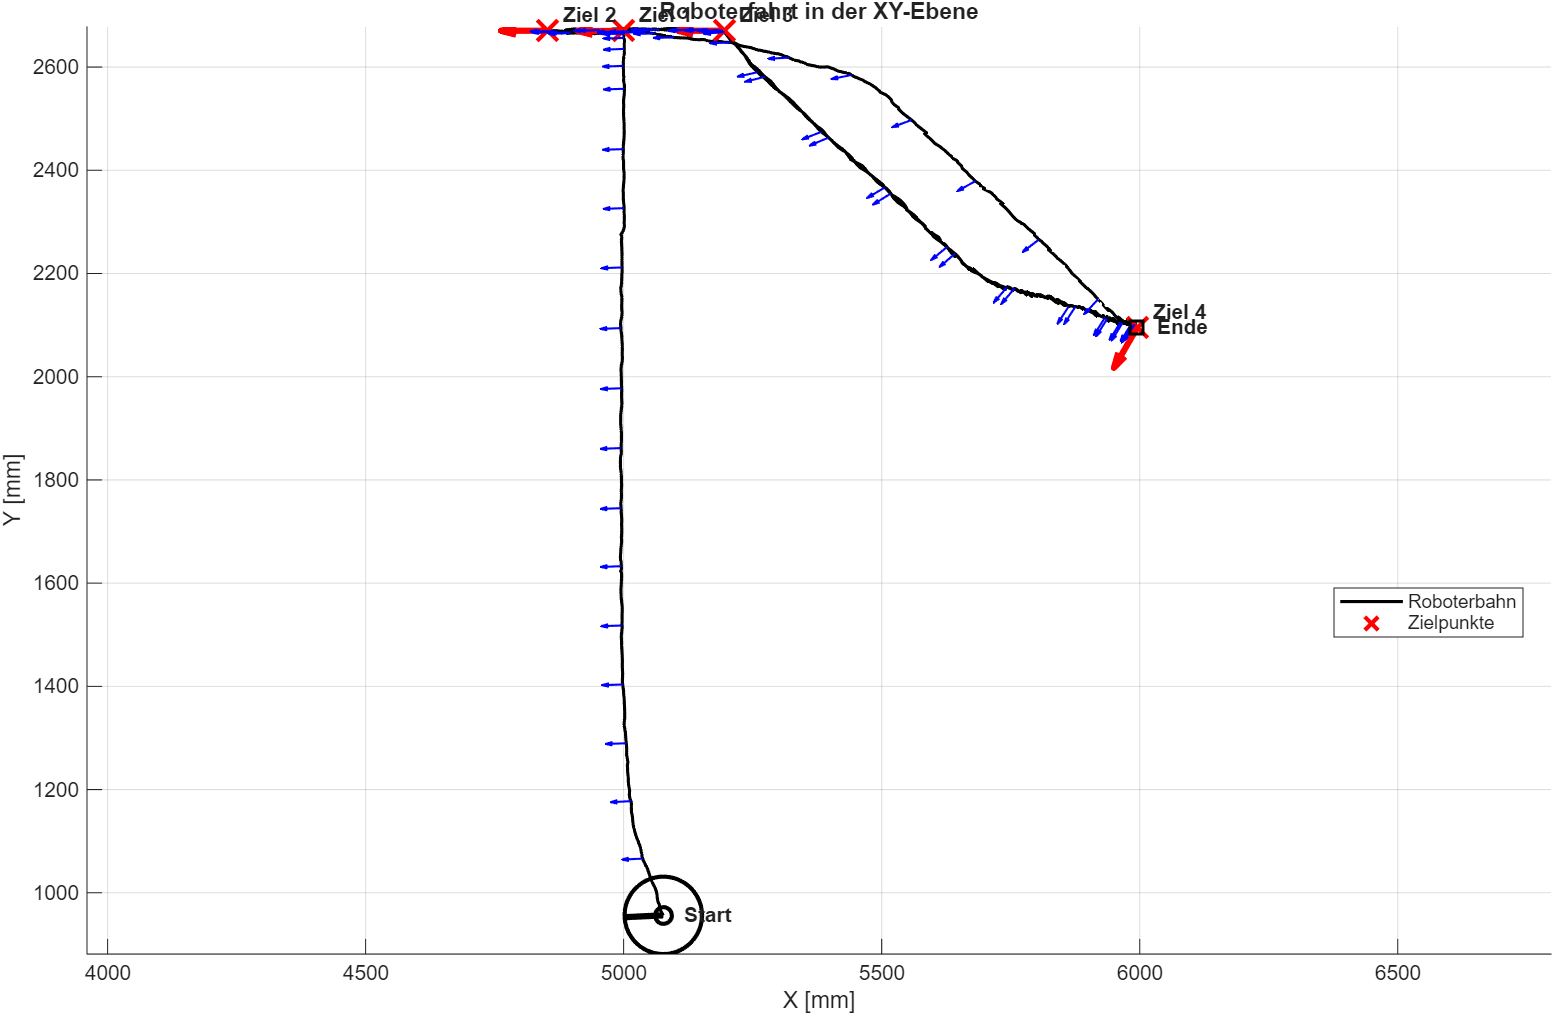
\includegraphics[width=0.95\textwidth]{_Bilder/ablagepunkt_xy}
    \caption{Rekonstruierte Roboterfahrt in der XY-Ebene mit Richtungspfeilen.}
    \label{fig:ablagepunkt_xy}
\end{figure}

Abbildung~\ref{fig:ablagepunkt_xy} zeigt die rekonstruierte Roboterfahrt in der XY-Ebene. Die Darstellung ist Analog wie die in Abbildung~\ref{fig:reale_positionsfahrt_xy} .Zur Veranschaulichung der Positionsgenauigkeit ist in Abbildung~\ref{fig:ablagepunkt_x} zusätzlich der Verlauf der x-Position über der Zeit dargestellt. Die eingezeichneten Sollpositionen sowie die zulässigen Toleranzbereiche verdeutlichen, dass der Roboter den Ablagepunkt innerhalb der geforderten Genauigkeit erreicht und stabil hält.

\begin{figure}[H]
    \centering
    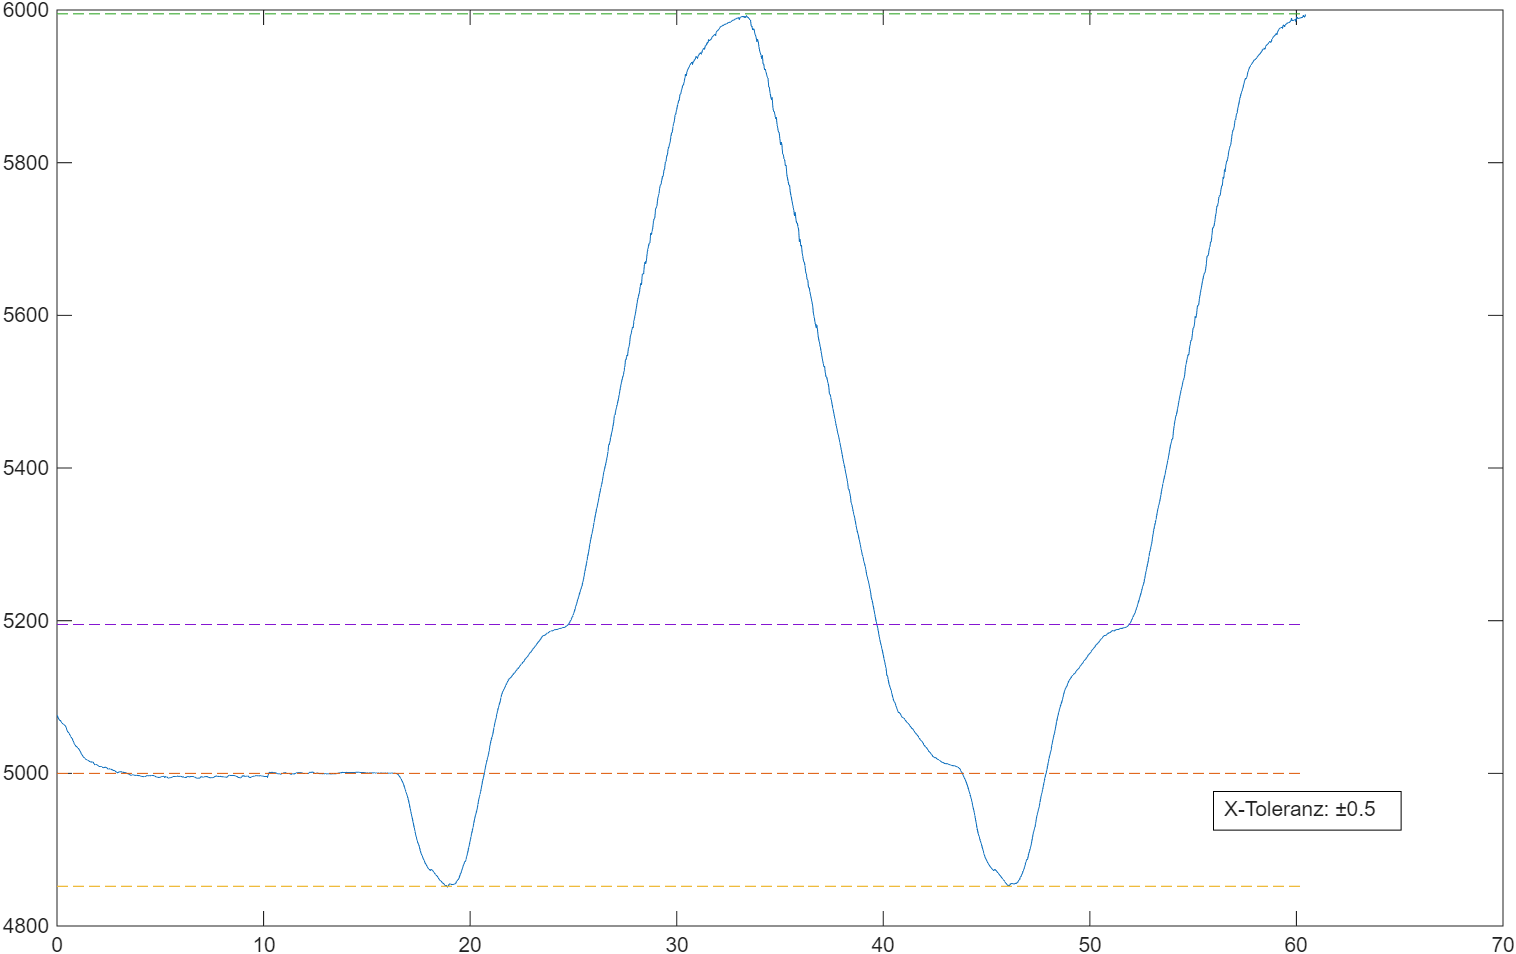
\includegraphics[width=0.9\textwidth]{_Bilder/ablagepunkt_x_verlauf}
    \caption{Weiterer X-Verlauf einer aufgezeichneten Fahrt mit Zielniveaus und Toleranzhinweis.}
    \label{fig:ablagepunkt_x}
\end{figure}

Die Versuchsergebnisse zeigen, dass der entwickelte Fuzzy-Regler auch bei erhöhten Genauigkeitsanforderungen zuverlässig arbeitet. Der Ablagepunkt wurde  innerhalb der vorgegebenen Positions- und Orientierungstoleranzen angefahren. Während der Versuche traten weder Kollisionen noch instabile Regelvorgänge auf. Damit konnte nachgewiesen werden, dass sich der entwickelte Regler sowohl für allgemeine Positionsfahrten als auch für präzise Positionieraufgaben im praktischen Einsatz eignet.

\section{Vergleich zwischen Simulation und realem System}

Die im Rahmen der Simulation ermittelten Reglerparameter stellten eine sehr gute Ausgangsbasis für die Inbetriebnahme des realen Systems dar. Dennoch zeigte sich, dass eine geringfügige Nachjustierung einzelner Skalierungsparameter erforderlich war. Der wichtigste Unterschied zwischen Simulation und realem System liegt in der Modelltreue. Während in der Simulation ausschließlich das kinematische Verhalten des Roboters berücksichtigt wird, treten im realen System zusätzlich dynamische Effekte wie Massenträgheit, Reibung, Radschlupf, mechanische Toleranzen sowie Messrauschen auf. Insbesondere im Bereich der Ablageposition spielt außerdem die vorhandene Federung eine wichtige Rolle. Um den Zielpunkt zuverlässig zu erreichen, muss der Roboter mit einer geringen Restgeschwindigkeit in die federnd gelagerte Position einfahren. Dieses Verhalten wird im verwendeten Simulationsmodell nicht berücksichtigt und machte daher eine Feinabstimmung der Parameter am realen System erforderlich. Insgesamt zeigte sich jedoch, dass die Simulation ihren Zweck erfüllt hat. 

\section{Bewertung des Ergebniss}

Im Rahmen dieser Arbeit wurde ein Fuzzy-Regler für einen omnidirektionalen Roboter entwickelt, simuliert und erfolgreich in die bestehende Robotersteuerung integriert. Ziel war es, eine einheitliche Reglerstruktur zu schaffen, die sowohl für Positionsfahrten als auch als Grundlage für zukünftige Vektorfahrten verwendet werden kann. Die Simulation ermöglichte eine automatische Bestimmung geeigneter Skalierungsparameter und zeigte sich als gut geeignet. Die anschließenden Fahrversuche zeigten, dass der Regler Zielpositionen und Zielorientierungen zuverlässig anfährt und auch bei engen Toleranzen ein stabiles Regelverhalten erreicht. Kleinere Anpassungen der Simulationsparameter waren aufgrund realer Einflüsse wie mechanischer Toleranzen und der Federung im Bereich der Ablageposition erforderlich, änderten jedoch nichts am grundsätzlichen Erfolg des entwickelten Regelungskonzepts. Besonders vorteilhaft erwiesen sich der modulare Aufbau des Reglers, die übersichtliche Regelbasis sowie die Möglichkeit, dieselbe Reglerstruktur sowohl für Positions- als auch für Vektorfahrten zu verwenden. Die Parametrierung erfolgt ausschließlich über wenige Skalierungsparameter und kann dadurch einfach an unterschiedliche Anforderungen angepasst werden. Insgesamt konnten die zu Beginn formulierten Ziele erreicht werden. Der entwickelte Fuzzy-Regler stellt eine robuste und gut nachvollziehbare Lösung für die Regelung des omnidirektionalen Roboters dar und bildet eine geeignete Grundlage für zukünftige Erweiterungen. Für zukünftige Arbeiten bietet sich insbesondere eine Erweiterung der Simulation um ein dynamisches Robotermodell an. Darüber hinaus könnten weitere Reglerparameter, beispielsweise die Zugehörigkeitsfunktionen oder die Regelbasis selbst, automatisch optimiert sowie unterschiedliche Fahrszenarien gleichzeitig zur Parametrierung herangezogen werden. Ebenso stellt die Umsetzung einer kontinuierlichen Vektorfahrt durch gleitende Zielpunkte einen vielversprechenden nächsten Entwicklungsschritt dar.